\documentclass[11pt]{article}
\usepackage[a4paper,margin=25mm]{geometry}
\usepackage[T1]{fontenc}
\usepackage{lmodern}
\usepackage{booktabs}
\usepackage{amsmath}
\usepackage{graphicx}
\usepackage{hyperref}
\usepackage{xcolor}
\newcommand{\code}[1]{\texttt{#1}}
\newcommand{\us}{\textmu s}
\graphicspath{{figs/}}

\title{The seed-channel correction of the light collection}
\author{BGOTSCAN}
\date{2026-10-15}

\begin{document}
\maketitle

\section{The problem}

The equalized sum of the channels with positive charge, $Q^{\rm eq}_0$,
gives a 511~keV line 38\% wide (FWHM over peak) on the run
\code{195K\_41V\_th20}, with a noise term of 17\% measured on the control
charges. The remaining 34\% is not the crystal. The photopeak position of
the events grouped by the channel that collected most light spreads by
11\% rms, from 0.81 to 1.26 of the median, and the spread follows the map
of the array: the lowest positions ring the block of twelve dead channels,
the highest lie far from it. An interaction next to the block loses 15 to
25\% of its light. A spread of 11\% rms is by itself a 26\% FWHM term, and
in quadrature with the noise and an intrinsic 12 to 15\% it accounts for
the 38\%.

Seen directly: the events whose seed channel is 12~mm or more from the
block give a line 22\% wide at 674\,400 ADC\,ns, those next to it a line
31\% wide at 574\,700. The whole sample is these populations on top of
each other, 15\% apart.

\section{The correction}

For an event $e$ with channel charges $q_c$ and gain factors $g_c$ from
the single-photoelectron table, over the live channels $c$:

\begin{enumerate}
\item The equalized charges, and the seed channel, the one with the
  largest of them:
  \[
    q^{\rm eq}_c = \frac{q_c}{g_c}, \qquad
    s(e) = \text{the } c \text{ with the largest } q^{\rm eq}_c .
  \]
\item The sum over the channels with positive charge:
  \[
    Q^{\rm eq}_0(e) = \sum_{c\,:\; q_c > 0} q^{\rm eq}_c .
  \]
\item For every channel $k$ that is the seed of at least 40 events, the
  photopeak position of those events:
  \[
    \mu_k = \text{peak of the histogram of } Q^{\rm eq}_0(e)
    \text{ over the events with } s(e) = k .
  \]
  Figure~\ref{fig:map}, left, is the map of the $\mu_k$ in units of
  their median.
\item The factor, and the corrected charge:
  \[
    f_k = \frac{\mu_k}{\operatorname{median}_k \mu_k}, \qquad
    Q^{\rm pos}_0(e) = \frac{Q^{\rm eq}_0(e)}{f_{s(e)}} .
  \]
\end{enumerate}

An event whose seed is channel 24, next to the block, has its total
divided by $f_{24} = 0.81$; the seed-24 events, which peaked at 0.81 of
the median, now peak at the median. The seed-51 events, which peaked at
1.26, are divided by 1.26 and land on the median too. Every population is
moved to the same place and the line is their superposition, aligned.
Events whose seed channel has fewer than 40 events keep $Q^{\rm eq}_0$:
388 of 4115 on this run.

The factor is a property of where the light fell, to the granularity of
one SiPM: it says nothing of the depth of the interaction, nor of where
within the 6~mm of the seed channel the light fell. It is measured on the
run itself, from the 511~keV line, so it absorbs whatever makes the
collection depend on the position: the dead block, the Teflon wrapping,
the gain errors of the equalization table.

\section{Step by step}

\begin{figure}[htb]
\centering
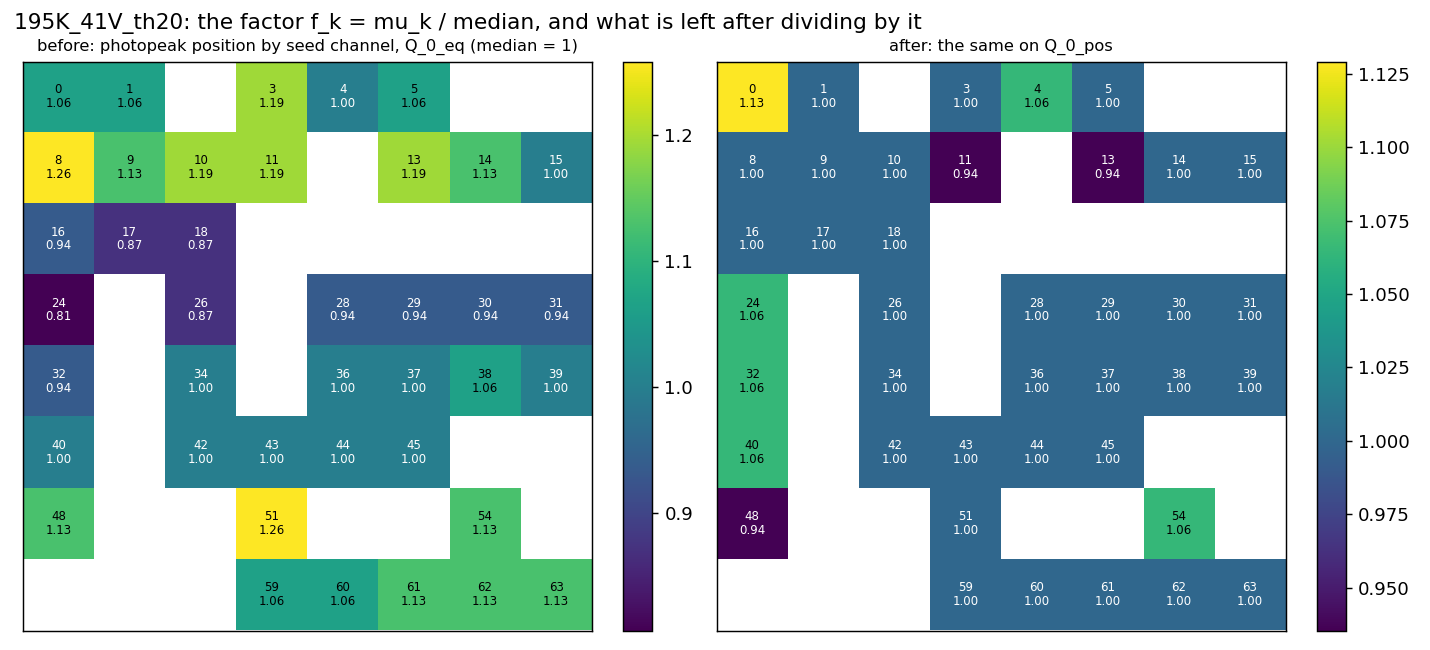
\includegraphics[width=\textwidth]{q0corr_195K_seedmap}
\caption{Left: the photopeak position of the events by seed channel,
$\mu_k$ over its median, on $Q^{\rm eq}_0$. The ring of the dead block
(16, 17, 18, 24, 26, 28 to 32) is at 0.81 to 0.94, the far channels (3,
8, 10, 11, 13, 51) at 1.19 to 1.26. Right: the same measurement repeated
on $Q^{\rm pos}_0$.}
\label{fig:map}
\end{figure}

\begin{figure}[htb]
\centering
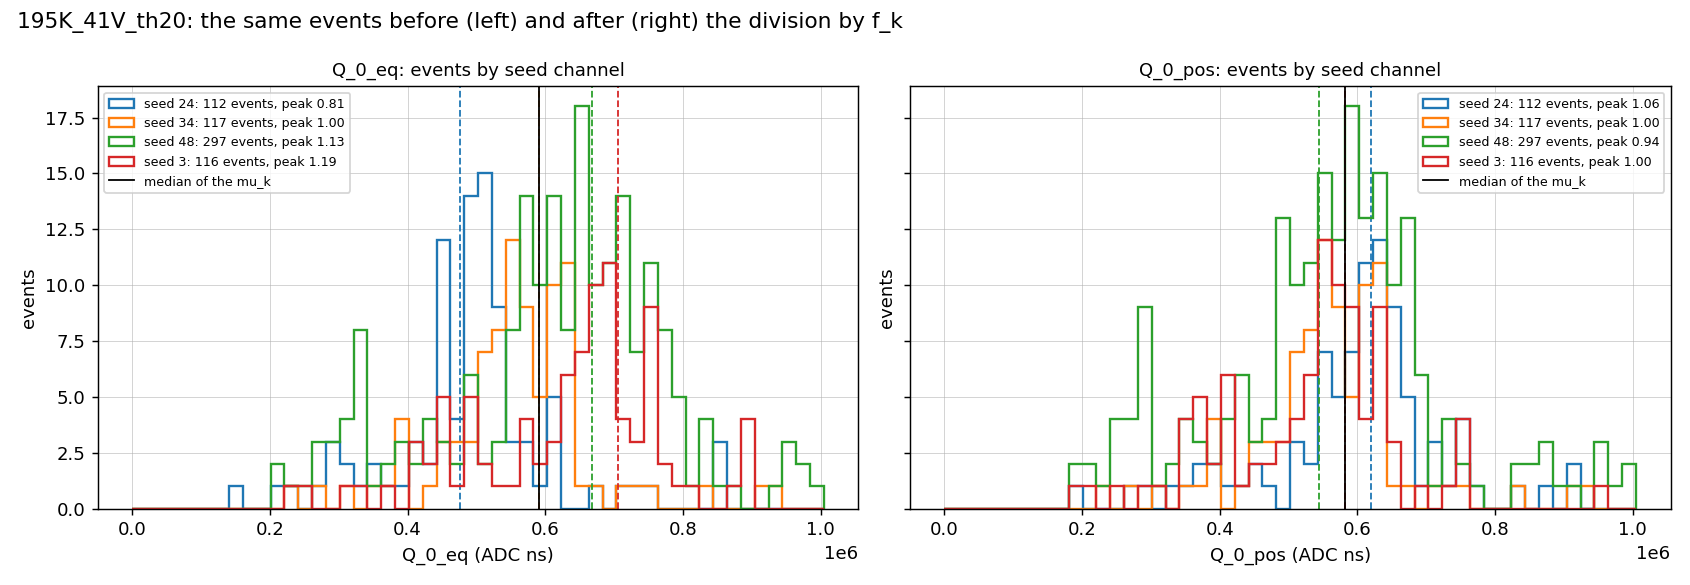
\includegraphics[width=\textwidth]{q0corr_195K_seeds}
\caption{Four seed-channel populations: 24 next to the block (0.81), 34
at the median (1.00), 48 (1.13) and 3 (1.19). Left, on $Q^{\rm eq}_0$,
each with its $\mu_k$ dashed and the median in black; right, the same
events on $Q^{\rm pos}_0$.}
\label{fig:seeds}
\end{figure}

\begin{figure}[htb]
\centering
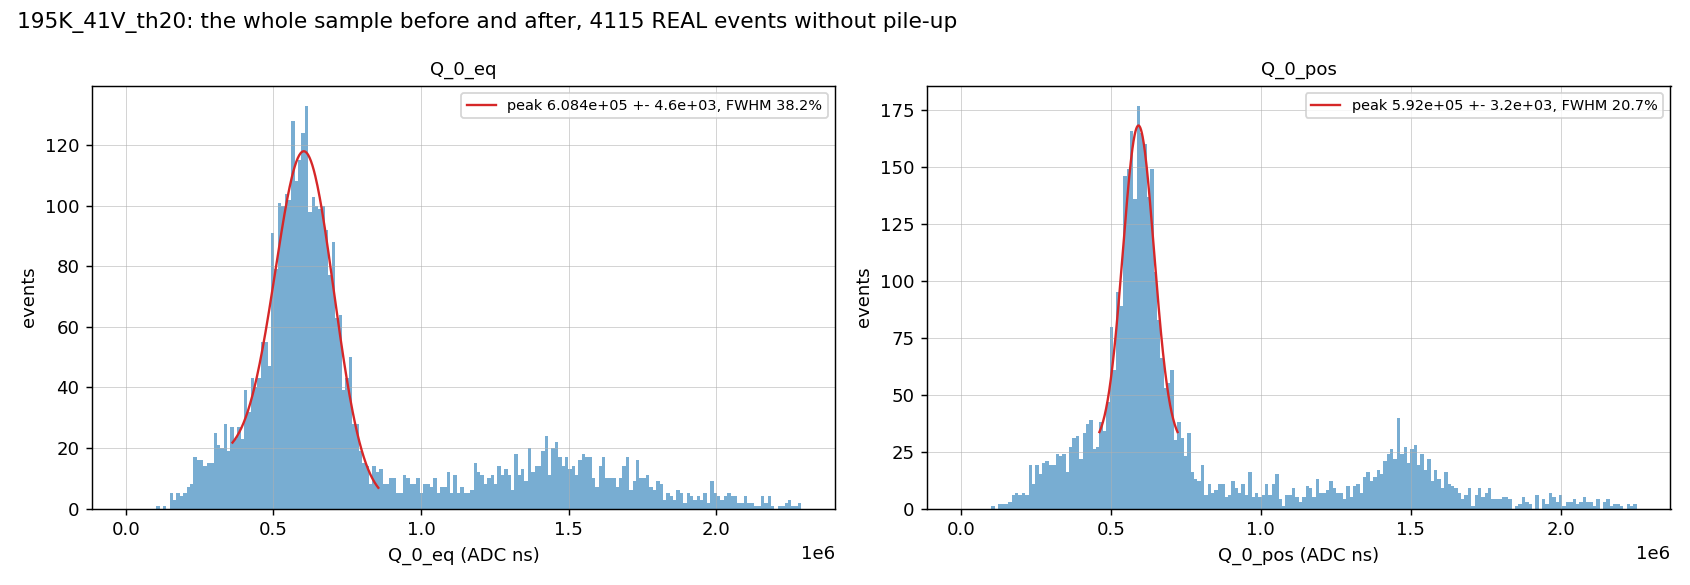
\includegraphics[width=\textwidth]{q0corr_195K_spectra}
\caption{The whole sample, 4115 REAL events without pile-up, before and
after: $Q^{\rm eq}_0$ at 608\,400 $\pm$ 4600 ADC\,ns, 38.2\% FWHM, and
$Q^{\rm pos}_0$ at 592\,000 $\pm$ 3200, 20.7\%.}
\label{fig:spectra}
\end{figure}

Figure~\ref{fig:map} is the factor, and what is left of the spread once
it is applied: 0.109 rms before, 0.035 after, the range 0.81 to 1.26
before and 0.94 to 1.13 after. Figure~\ref{fig:seeds} shows the
alignment on four populations, and figure~\ref{fig:spectra} the result on
the whole line, 38.2\% to 20.7\%.

A check that does not follow by construction: the 1275~keV line, which
the factor never used, is a smeared bump on $Q^{\rm eq}_0$ and a resolved
peak on $Q^{\rm pos}_0$ at 2.5 times the 511~keV position (the spectra
figure of \code{offline.py}).

\section{Limits}

\begin{itemize}
\item \textbf{Granularity of the factor.} $\mu_k$ is the centre of the
  highest bin of a 60-bin histogram, 6\% of the peak wide: the positions
  come in steps of 0.06 (0.81, 0.87, 0.94, 1.00, \dots), and after the
  correction the re-measured positions scatter by 0.035 rms, one bin.
  This is a term of about 8\% FWHM left in $Q^{\rm pos}_0$ by the
  method itself. With 40 to 300 events per seed channel, a Gaussian fit
  of each peak, or the interpolated mode, would remove most of it.
\item \textbf{Within one seed channel.} The width of a single population
  is 15 to 45\%, median 29\%, with the 17\% of noise inside: the
  collection varies across the 6~mm of one SiPM and the 20~mm of depth,
  and the factor cannot see it.
\item \textbf{The noise term.} $Q^{\rm pos}_0$ sums the positive channels
  only; the noise term from the control charges summed over the same
  channels is an overestimate for a masked sum (the mask keeps the
  channels whose noise came out positive, whose fluctuation is smaller
  than a full noise sample). The remainder after subtraction, 11.9\% at
  41~V, is a lower bound; at 40.5~V the term equals the width. The exact
  term is measured by noise injection: the control charges added to the
  event charges, the estimator recomputed with its mask, the broadening
  of the line.
\item \textbf{The finer version.} Each channel $c$ with its own response
  $r_c$, the charge it collects in a photopeak event that lights it
  relative to the others, applied before the sum,
  $Q(e) = \sum_c q^{\rm eq}_c / r_c$, over all live channels and without
  mask: the position correction and an exact noise subtraction in one
  estimator. Not yet written.
\end{itemize}

Figures by \code{src/py/q0corr.py} (\code{docs/manual/q0corr\_doc.tex}):
\code{python3 src/py/q0corr.py 195K\_41V\_th20 --save 195K\_41V}.

\end{document}
